\newpage
\section{Ôn tập chương 4}
\def\thoigian{90}
\de{Đề số 1}{Chương IV. Nguyên hàm – Tích phân}


\ind{PHẦN I.} \inden{Câu trắc nghiệm nhiều phương án lựa chọn. Mỗi câu hỏi học sinh chỉ chọn một phương án.}\\
\setcounter{ex}{0}
\Opensolutionfile{ans}[ans/2D4-OTC-TN]

\begin{ex}%[2D4N1-2]
	[Thi Thử - 2025-So-Ba-Ria-VT]
	Một nguyên hàm của hàm số $f(x) = \dfrac{1}{x}$ với $x \neq 0$ là
	\choice
	{$-\dfrac{1}{x^2} + 1$}
	{$\ln x + 1$}
	{$x^{-1} + 1$}
	{\True $\ln|x| + 1$}
	\loigiai{
		Ta có $\displaystyle\int f(x) \mathrm{\,d}x = \displaystyle\int \dfrac{1}{x} \mathrm{\,d}x = \ln|x| + C$.\\
		Vậy một nguyên hàm của hàm số $f(x) = \dfrac{1}{x}$ với $x \neq 0$ là $\ln|x| + 1$ với $C = 1$.
	}
\end{ex}

\begin{ex}%[2D4N1-3]
	Nguyên hàm của hàm số $f(x)=\sin x$ là
	\choice
	{$-\sin x+C$}
	{\True $-\cos x+C$}
	{$\cos x+C$}
	{$\sin x+C$}
	\loigiai{
		Nguyên hàm của hàm số $f(x)=\sin x$ là $-\cos x+C$.
	}
	
\end{ex}

\begin{ex}%[2D4N1-4]
	Hàm số nào sau đây là một nguyên hàm của hàm số $f(x)=25^x$?
	\choice
	{$F_3 (x)=\dfrac{25^x}{\log 25}$}
	{$F_2 (x)=25^x \ln 25$}
	{$F_1 (x)=25^x$}
	{\True $F_4 (x)=\dfrac{25^x}{\ln 25}$}
	\loigiai{
		Vì $\left(\dfrac{25^x}{\ln 25} \right)'=\dfrac{1}{\ln 25}\cdot25^x\cdot\ln 25=25^x$ nên một nguyên hàm của hàm số $f(x)=25^x$ là $F_4 (x)=\dfrac{25^x}{\ln 25}$.
	}
	
\end{ex}

\begin{ex}%[2D4N1-2]
	Tìm $\displaystyle\displaystyle\int\left(3x^3+3x^2+3x+4 \right)\mathrm{\, d}x$.
	\choice
	{$\dfrac{3x^4}{4}+x^3+\dfrac{5x^2}{2}+4x+C$}
	{$\dfrac{3x^4}{4}+x^3+\dfrac{3x^2}{2}+11x+C$}
	{$9{x^2}+6x+3+C$}
	{\True $\dfrac{3x^4}{4}+{x^3}+\dfrac{3x^2}{2}+4x+C$}
	\loigiai{
		Ta có  $\displaystyle\displaystyle\int\left(3x^3+3x^2+3x+4 \right)\mathrm{\, d}x=\dfrac{3x^4}{4}+{x^3}+\dfrac{3x^2}{2}+4x+C$.
	}
\end{ex}

\begin{ex}%[2D4N2-1]
	Nếu $\displaystyle\int\limits_1^2f(x)\mathrm{\,d}x=-2$ và $\displaystyle\int\limits_2^3f(x)\mathrm{\,d}x=1$ thì $\displaystyle\int\limits_1^3f(x)\mathrm{\,d}x$ bằng
	\choice
	{\True $-1$}
	{$3$}
	{$-3$}
	{$1$}
	\loigiai{
		Áp dụng tính chất của tích phân, ta có\\ $$\displaystyle\int\limits_1^3f(x)\mathrm{\,d}x
		=\displaystyle\int\limits_1^2f(x)\mathrm{\,d}x
		+\displaystyle\int\limits_2^3f(x)\mathrm{\,d}x=-2+1=-1.$$
	}
	
\end{ex}
\begin{ex}%[2D4N2-2]%[2-TN-DS-TLN-THPT-HoNghinh-QuangNam-HKII-NH24-25]%[Lê Phúc]
	[THPT-HoNghinh-QuangNam-HKII-NH24-25]
	Tích phân $I=\displaystyle\int\limits_{-1}^1\left(x^3+3 x+2\right)\mathrm{\,d}x$ có giá trị là
	\choice
	{$I=3$}
	{$I=1$}
	{\True $I=4$}
	{$I=2$}
	\loigiai{Ta có $I=\displaystyle\int\limits_{-1}^1\left(x^3+3 x+2\right)\mathrm{\,d}x=\left(\dfrac{x^4}{4}+\dfrac{3x^2}{2}+2x\right)\Bigg |_{-1}^1=4$.}
\end{ex}

\begin{ex}%[2D4N2-2]
	[Thi thử THPT Văn Quán - Vĩnh Phúc- NH2024-2025]
	Cho hàm số $y=f(x)$ liên tục trên $\mathbb{R}$ và có một nguyên hàm là $F(x)$. Biết rằng $F(1)=9$, $F(2)=5$. Giá trị của biểu thức $\displaystyle\displaystyle\int\limits\limits_{1}^{2} f(x) \mathrm{\,d} x$ bằng
	\choice
	{$45$}
	{$14$}
	{$4$}
	{\True $-4$}
	\loigiai{
		Ta có $\displaystyle\displaystyle\int\limits\limits_{1}^{2} f(x) \mathrm{\,d} x=F(x)\Big|_{1} ^{2}=F(2)-F(1)=5-9=-4$.}
	
\end{ex}

\begin{ex}%[2D4H2-2]
	[Thi Thử - 2025-KHTN-HaNoi-lan2]
	Cho $\displaystyle\int\limits_0^2\left[f(x)-3x^2\right]\mathrm{\,d}x=4$. Tích phân $\displaystyle\int\limits_0^2f(x)\mathrm{\,d}x$ bằng
	\choice
	{$-4$}
	{$4$}
	{$8$}
	{\True $12$}
	\loigiai{
		Ta có
		\begin{eqnarray*}
			&&\displaystyle\int\limits_0^2\left[f(x)-3x^2\right]\mathrm{\,d}x=4\\
			&\Leftrightarrow&\displaystyle\int\limits_0^2f(x)\mathrm{\,d}x-3\displaystyle\int\limits_0^2x^2\mathrm{\,d}x=4\\
			&\Leftrightarrow&\displaystyle\int\limits_0^2f(x)\mathrm{\,d}x-x^3\bigg|_0^2=4\\
			&\Leftrightarrow&\displaystyle\int\limits_0^2f(x)\mathrm{\,d}x-8=4\\ &\Leftrightarrow&\displaystyle\int\limits_0^2f(x)\mathrm{\,d}x=12.
		\end{eqnarray*}
	}
\end{ex}

\begin{ex}%[2D4H3-2]
	Viết công thức tính diện tích $S$ của hình phẳng được giới hạn bởi đồ thị hàm số $y=f\left( x \right)$, trục $Ox$ và các đường thẳng $x=a$, $x=b\left(a<b \right)$.
	\choice
	{$S=\displaystyle\int\limits_a^b{f^2\left( x \right)\mathrm{d}x}$}
	{$S=\pi \displaystyle\int\limits_a^b{f\left( x \right)\mathrm{d}x}$}
	{\True $S=\displaystyle\int\limits_a^b{\left| f\left( x \right) \right| \mathrm{d}x}$}
	{$S=\displaystyle\int\limits_a^b{f\left( x \right)\mathrm{d}x}$}
	\loigiai{
	}
	
\end{ex}

\begin{ex}%[2D4H3-1]
	Diện tích hình phẳng giới hạn bởi hai đường $y=x^2-4$ và $y=2x-4$ bằng
	\choice
	{$\dfrac{4\pi}{3}$}
	{$36\pi$}
	{$36$}
	{\True $\dfrac{4}{3}$}
	\loigiai{
		Ta có phương trình hoành độ giao điểm của hai đường là $x^2-4=2x-4\Leftrightarrow \hoac{&x=0\\&x=2.}$\\
		Diện tích hình phẳng giới hạn bởi hai đường thẳng đã cho là
		$$\displaystyle\int\limits_0^2 \left|x^2-2x \right| \mathrm{\,d}x=\left|\left(\dfrac{x^3}{3}-x^2\right)\Bigg|_0^2\right|=\dfrac{4}{3}\text { (đvdt)}.$$
	}
	
\end{ex}

\begin{ex}%[Câu 11]%[2D4H3-3]
	[Thi Thử - 2025-KHTN-HaNoi-lan2]
	Cho hình phẳng $(H)$ giới hạn bởi đồ thị $y=2x-x^2$ và trục hoành. Thể tích vật thể tròn xoay sinh ra khi cho $(H)$ quay quanh trục hoành bằng
	\choice
	{$\dfrac{4\pi}{3}$}
	{\True $\dfrac{16\pi}{15}$}
	{$\dfrac{16}{15}$}
	{$\dfrac{4}{3}$}
	\loigiai{
		Phương trình hoành độ giao điểm của đồ thị $y=2x-x^2$ và trục hoành là
		$2x-x^2=0\Leftrightarrow \hoac{&x=0 \\&x=2.}$\\
		Thể tích vật thể tròn xoay sinh ra khi cho $(H)$ quay quanh trục hoành là
		$$V=\pi \displaystyle\int\limits_0^2\left(2x-x^2\right)^2\mathrm{\,d}x=\dfrac{16\pi}{15}.$$}
	
\end{ex}

\begin{ex}%[2D4H3-1]
	\immini {
		Cho hàm số $y=f(x)$ có đồ thị như hình vẽ. Biết các diện tích $S_1=\dfrac{7}{12}$ và $S_2=\dfrac{45}{4}$. Tính tích phân $I=\displaystyle\int \limits_{-1}^3f (x)dx$.
		\choice[2]
		{$I=-\dfrac{71}{6}$}
		{$I=\dfrac{32}{3}$}
		{\True $I=-\dfrac{32}{3}$}
		{$I=\dfrac{71}{6}$}
	}{
		\begin{tikzpicture}[scale=0.6, font=\footnotesize, line join=round, line cap=round, >=stealth]
			\draw[->] (-2,0) --(4,0)node[below left] {$x$};
			\draw[->] (0,-4.8) -- (0,2)node[right] {$y$};
			\draw [fill=black] (0,0) circle(1pt) node[below left] {$O$};
			\begin{scope}
				\clip (-2,-4.8) rectangle (4,2);
				\draw[smooth,black,thick,samples=200,domain=-2:4] plot(\x,{(3/4)*(\x)^3-(3/2)*(\x)^2-(9/4)*(\x)});
				\filldraw [pattern=north west lines, opacity=0.5]
				plot[smooth,black,thick,samples=200,domain=-1:3] (\x,{(3/4)*(\x)^3-(3/2)*(\x)^2-(9/4)*(\x)})--(3,0)--(-1,0) ;
			\end{scope}
			\foreach \x/\g in {-1/135,3/45}
			\draw [fill=black] (\x,0) circle(1pt) + (\g:4mm) node {$\x$};
			\path (-0.5,0.3)node[]{$S_1$}
			(2,-2.5)node[above]{$S_2$};
		\end{tikzpicture}
	}
	\loigiai{
		Ta có $$I=\displaystyle\int\limits_{-1}^3f (x)\mathrm{~d}x=\displaystyle\int\limits_{-1}^0 f (x)\mathrm{d}x+\displaystyle\int\limits_0^3 f (x)\mathrm{d}x=S_1-S_2=\dfrac{7}{12}-\dfrac{45}{4}=-\dfrac{32}{3}.$$
	}
	
\end{ex}
\Closesolutionfile{ans}
\indapan{4}{ans/2D4-OTC-TN}

\ind{PHẦN II.} \inden{Câu trắc nghiệm đúng sai. Trong mỗi ý a), b), c), d) ở mỗi câu, học sinh chọn đúng hoặc sai.}\\
\setcounter{ex}{0}
\Opensolutionfile{ans}[ans/2D4-OTC-DS]
\begin{ex}%[2D4H2-2]
	[Thi Thử - 2025-So-Hai-Duong]
	Cho hàm số $y=f(x)$ liên tục trên $\mathbb{R}$ và thỏa mãn $\displaystyle\int\limits_1^3f(x)\mathrm{\,d}x=2$.
	\choiceTF
	{\True $\displaystyle\int\limits_1^33f(x)\mathrm{\,d}x=6$}
	{Nếu $\displaystyle\int\limits_2^3f(x)\mathrm{\,d}x=-1$ thì $\displaystyle\int\limits_1^2f(x)\mathrm{\,d}x=1$}
	{Nếu $F(x)$ là một nguyên hàm của $f(x)$ trên đoạn $\left[1;3\right]$ thỏa mãn $F(1)=3$ thì $F(3)=1$}
	{\True $\displaystyle\int\limits_1^3\dfrac{xf(x)+x^2-1}{x} \mathrm{\,d}x=a+b\ln 3$, $\left(a\in \mathbb{Q},b\in \mathbb{Q}\right)$. Ta có $a+b=5$}
	\loigiai{
		\begin{itemchoice}
			\itemch Ta có  $\displaystyle\int\limits_1^33f(x)\mathrm{\,d}x=3\displaystyle\int\limits_1^3f(x)\mathrm{\,d}x=3\cdot 2=6$.
			\itemch Ta có  $\displaystyle\int\limits_1^2f(x)\mathrm{\,d}x=\displaystyle\int\limits_1^3f(x)\mathrm{\,d}x-\displaystyle\int\limits_2^3f(x)\mathrm{\,d}x=2-\left(-1\right)=3$.
			\itemch Ta có  $\displaystyle\int\limits_1^3f(x)\mathrm{\,d}x=F(3)-F(1)$. Suy ra $F(3)-F(1)=2\Rightarrow F(3)=3+2=5$.
			\itemch Ta có \begin{eqnarray*}
				\displaystyle\int\limits_1^3\dfrac{xf(x)+x^2-1}{x} \mathrm{\,d}x&=&\displaystyle\int\limits_1^3\left[f(x)+x-\dfrac{1}{x} \right]\mathrm{\,d}x\\
				&=&\displaystyle\int\limits_1^3f(x)\mathrm{\,d}x+\displaystyle\int\limits_1^3x\mathrm{\,d}x-\displaystyle\int\limits_1^3\dfrac{1}{x} \mathrm{\,d}x\\
				&=&2+\left. \dfrac{x^2}{2} \right|_1^3-\left. \ln \left|x\right|\right|_1^3=2+4-\ln 3\\
				&=&6-\ln 3.
			\end{eqnarray*}
			Vậy $a=6$, $b=-1\Rightarrow a+b=5$.
		\end{itemchoice}
	}
	
\end{ex}
\begin{ex}%[2D4V3-2]
	[Thi Thử - 2025-ChuyenKHTN-HaNoi-Lan1]
	Một công ty thiết kế mẫu huy hiệu để tặng cho khách hàng thân thiết của mình (xem hình vẽ bên dưới). Trong đó $ABCD$ là hình vuông có cạnh bằng $4$ cm, các đường cong $AOD$ và $BOC$ là một phần của các parabol đỉnh $O$. Với hệ trục tọa độ $Oxy$ (đơn vị trên mỗi trục tọa độ là cen-timet) thì điểm $A$ có tung độ bằng $1$. Biết phần tô đậm trong hình vẽ được phủ vàng với chi phí $1$ một triệu đồng /$1$ cm$^2$, phần còn lại được phủ bạc với chi phí $300$ nghìn đồng/$1$ cm$^2$, các chi phí còn lại là $500$ nghìn đồng
	\immini{\choiceTF
		{\True Parabol chứa đường cong $BOC$ có phương trình là $\break y=-\dfrac{3}{4} x^2$}
		{Parabol chứa đuờng cong $AOD$ có phương trình là $\break y=\dfrac{1}{16} x^2$}
		{ Diện tích phần tô đậm trong hình vẽ lớn hơn $5{,}5$ cm$^2$}
		{\True Chí sản xuất $1$ chiếc huy hiệu trên nhỏ hơn $9$ triệu đồng}
		}
	{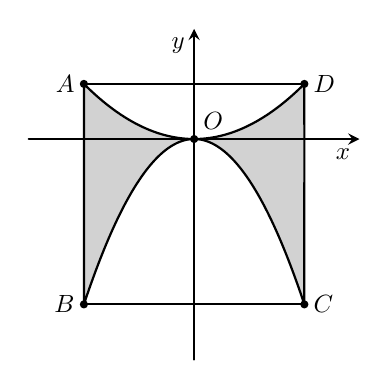
\begin{tikzpicture}[line join=round, line cap=round,>=stealth,thick,scale=.7]
			\tikzset{every node/.style={scale=0.9}}
			\begin{scope}
				\draw[fill=gray!35](-2,0)--plot[samples=200,domain=-2:2,smooth,variable=\x] (\x,{0.25*(\x)^2})--(2,0);
				\draw[fill=gray!35](-2,0)--plot[samples=200,domain=-2:2,smooth,variable=\x] (\x,{-0.75*(\x)^2})--(2,0);
				\draw[fill=black](-2,1) circle (1.5pt) node[left]{$A$} (-2,-3) circle (1.5pt) node[left]{$B$} (2,-3) circle (1.5pt) node[right]{$C$} (2,1) circle (1.5pt) node[right]{$D$} (0,0) circle (1.5pt) node[above right]{$O$};
				\draw (-2,1)--(2,1) (2,-3)--(-2,-3);
			\end{scope}
			\draw[->] (-3,0)--(3,0) node[below left] {$x$};
			\draw[->] (0,-4)--(0,2) node[below left] {$y$};
	\end{tikzpicture}}
	\loigiai{
		\begin{center}
			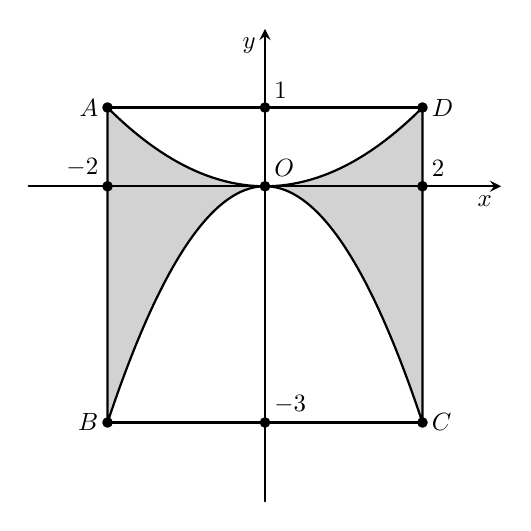
\begin{tikzpicture}[line join=round, line cap=round,>=stealth,thick,scale=1]
				\tikzset{every node/.style={scale=0.9}}
				\begin{scope}
					\draw[fill=gray!35](-2,0)--plot[samples=200,domain=-2:2,smooth,variable=\x] (\x,{0.25*(\x)^2})--(2,0);
					\draw[fill=gray!35](-2,0)--plot[samples=200,domain=-2:2,smooth,variable=\x] (\x,{-0.75*(\x)^2})--(2,0);
					\draw[fill=black](-2,1) circle (1.5pt) node[left]{$A$} (-2,-3) circle (1.5pt) node[left]{$B$} (2,-3) circle (1.5pt) node[right]{$C$} (2,1) circle (1.5pt) node[right]{$D$} (0,0) circle (1.5pt) node[above right]{$O$} (2,0) circle (1.5pt) node[above right]{$2$} (-2,0) circle (1.5pt) node[above left]{$-2$} (0,1) circle (1.5pt) node[above right]{$1$} (0,-3) circle (1.5pt) node[above right]{$-3$};
					\draw (-2,1)--(2,1) (2,-3)--(-2,-3);
				\end{scope}
				\draw[->] (-3,0)--(3,0) node[below left] {$x$};
				\draw[->] (0,-4)--(0,2) node[below left] {$y$};
			\end{tikzpicture}
		\end{center}
		\begin{itemchoice}
			\itemch Gọi parabol chứa đường cong $BOC$ có phương trình là $y=a_1x^2$.\\
			Vì parabol đi qua điểm $C(2;-3)$ nên ta có $-3=a_1\cdot2^2\Leftrightarrow a_1=\dfrac{-3}{4} \Rightarrow y=\dfrac{-3}{4} x^2$.
			\itemch Gọi parabol chứa đường cong $AOD$ có phương trình là $y=a x^2$.\\
			Vì Parabol đi qua điểm $A(-2; 1)$ nên ta có $1=a(-2)^2\Leftrightarrow a=\dfrac{1}{4} \Rightarrow y=\dfrac{1}{4} x^2$.
			\itemch Diện tích phần tô đậm là 
			$$S_1=\displaystyle\int\limits_{-2}^2\left(\dfrac{x^2}{4}+\dfrac{3x^2}{4}\right)\mathrm{\, d}x=\dfrac{16}{3}\left(\mathrm{cm}^2\right).$$
			Vậy $S_1<5{,}5$.
			\itemch Diện tích hình vuông $ABCD$ là $S_{h v}=4\cdot4=16$ cm$^2$.\\
			Diện tích phần không tô đậm
			$S_k=16-\dfrac{16}{3}=\dfrac{32}{3}$ cm$^2$.\\
			Tổng chi phí để làm chiếc huy hiệu
			$$T=100\,0000\cdot \dfrac{32}{3}+300\,000\cdot \dfrac{16}{3} \approx 8\,533\,000.$$
			Giá trị này nhỏ hơn $9$ triệu đồng.
			
		\end{itemchoice}
	}
\end{ex}

\Closesolutionfile{ans}
\indapan{2}{ans/2D4-OTC-DS}

\ind{PHẦN III.} \inden{Câu trắc nghiệm trả lời ngắn.}
\setcounter{ex}{0}
\Opensolutionfile{ans}[ans/2D4-OTC-TLN]
\begin{ex}%[2D4H2-2]
	[Kiểm tra Toán 12 HKII năm học 2024 - 2025-THPT Ngô Gia Tự - Phú Yên]
	Biết tích phân $\displaystyle \int \limits _1^{\mathrm{e}} \left(1-\dfrac{1}{x}\right) \mathrm{\,d}x=\mathrm{e}+a$. Giá trị của $a$ bằng bao nhiêu?
	\shortans[oly]{$-2$}
	\loigiai{Ta có $\displaystyle \int \limits _1^{\mathrm{e}} \left(1-\dfrac{1}{x}\right) \mathrm{\,d}x=\left(x-\ln x\right)\bigg|_1^{\mathrm{e}}=\mathrm{e}-\ln \mathrm{e} -1 + \ln 1=\mathrm{e} -2$.\\ 
	Vậy	$a=-2$.
	}
\end{ex}
\begin{ex}%[2D4H3-3]
	[Kiểm tra Toán 12 HKII NH24-25-THPT Hoàng Hoa Thám-TPHCM]
	Người ta tạo ra mô hình một quả trứng ngỗng bằng cách quay hình phẳng giới hạn bởi đồ thị hàm số $y=\dfrac{1}{30} \sqrt{7\,569-400x^2}$ và trục hoành với $-4{,}35 \le x \le 4{,}35$ quanh trục $Ox$. Sử dụng mô hình này để tính thể tích quả trứng theo đơn vị cm$^3$ và làm tròn đến hàng đơn vị (với $x$, $y$ được đo theo đơn vị cm).
	\shortans[oly]{153}
	\loigiai{Thể tích quả trứng là thể tích của khối tròn xoay được tạo thành khi quay hình phẳng tạo bởi đồ thị của hàm số $y=\dfrac{1}{30} \sqrt{7\,569-400x^2}$, trục hoành và hai đường thẳng $x=-4{,}35$ và $x=4{,}35$ quanh trục hoành. Do đó
		$$V=\pi \displaystyle \int \limits_{-4{,}35}^{4{,}35} \left(\dfrac{1}{30} \sqrt{7\,569-400x^2}\right)^2 \mathrm{\,d}x=\dfrac{24\,389 \pi}{500} \approx 153 \; \text{(cm$^3$)}.$$}
\end{ex}
\begin{ex}%[2D4V3-3]
	Hình dưới mô phỏng phần bên trong của một chậu cây có dạng khối tròn xoay tạo thành khi quay một phần của đồ thị hàm số $y=\sqrt{x}+\dfrac{3}{2}$ với $0\le x\le 4$ quanh trục hoành. Tính thể tích phần bên trong (dung tích) của chậu cây, biết đơn vị trên các trục $O x$, $O y$ là decimét \textit{(kết quả làm tròn đến hàng đơn vị)}.
	\begin{center}
		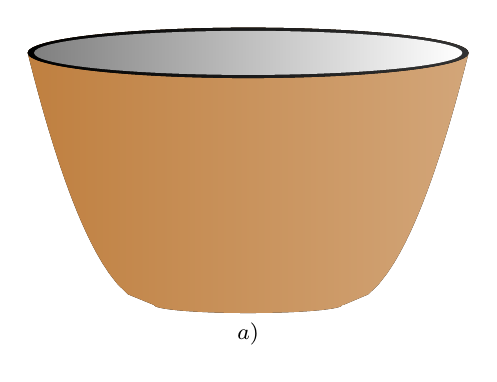
\begin{tikzpicture}[scale=0.8, font=\footnotesize, line join=round, line cap=round,>=stealth]
			\begin{scope}[rotate=90]
				\fill[left color=brown,right color=brown!70, draw=none] (0,-3/2) arc (-90:-270: 0.13 and 1.5)--(0,3/2)--plot[domain=0:4](\x,{sqrt(\x)+3/2})--(4,3.5)arc (90:-90: 0.4 and 3.5)--(4,-3.5)--plot[domain=4:0](\x,{-sqrt(\x)-3/2})--cycle;
				\fill[left color=black,right color=black!80,draw=none] (4,0) ellipse (0.4 and 3.5);
				\fill[left color=black!50,right color=white,draw=none] (4,0) ellipse (0.35 and 3.4);
			\end{scope}
			\node[below] at (current bounding box.south){$a)$};
		\end{tikzpicture}
		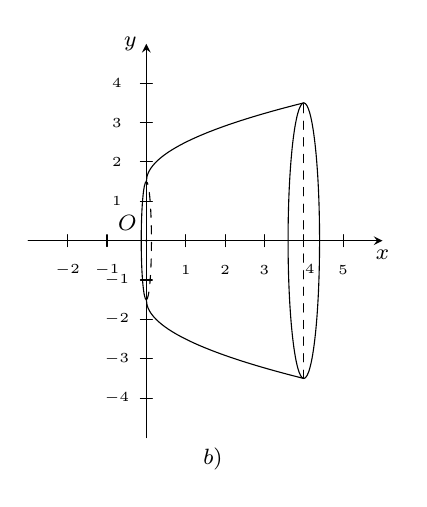
\begin{tikzpicture}[scale=0.5, font=\footnotesize, line join=round, line cap=round,>=stealth]
			%\fill[color=cyan!70, draw=none] (0,-3/2)--(0,3/2)--plot[domain=0:4](\x,{sqrt(\x)+3/2})--(4,3.5)--(4,-3.5)--plot[domain=4:0](\x,{-sqrt(\x)-3/2})--cycle;
			\draw[->] (-3,0) --(6,0) node[below]{$x$};
			\draw[->] (0,-5) --(0,5) node[left]{$y$};
			\fill (0,0) node[above left]{$O$} circle (1pt);
			\draw[smooth,samples=200,domain=0:4] plot(\x,{sqrt(\x)+3/2});
			\draw[smooth,samples=200,domain=0:4] plot(\x,{-sqrt(\x)-3/2});
			\draw (4,0) ellipse (0.4 and 3.5);
			\draw (0,3/2) arc (90:270: 0.13 and 1.5);
			\draw[dashed] (0,-3/2) arc (-90:90: 0.13 and 1.5);
			\draw[dashed] (4,-7/2)--(4,7/2);
			\foreach \x in {-4,-3,-2,-1,1,2,3,4}
			\draw (0.15,\x)--(-0.15,\x) node[shift={(180:3mm)},font=\tiny]{$\x$};
			\foreach \x in {-2,-1,1,2,3,5}
			\draw (\x,0.15)--(\x,-0.15) node[shift={(-90:3mm)},font=\tiny]{$\x$};
			\foreach \x in {4}
			\draw (\x,0.15)--(\x,-0.15) node[shift={(-75:3mm)},font=\tiny]{$\x$};
			\node[below] at (current bounding box.south){$b)$};
		\end{tikzpicture}
	\end{center}
	\shortans[oly]{$104$}
	\loigiai{
		Thể tích bên trong lòng chậu cây đó là 
		\[V=\pi\displaystyle\int\limits_0^4\left(\sqrt{x}+\dfrac{3}{2}\right)^2\mathrm{\, d}x=\pi\displaystyle\int\limits_0^4\left(x+3 \sqrt{x}+\dfrac{9}{4}\right)\mathrm{\, d}x=\left.\pi\left(\dfrac{x^2}{2}+2 x^{\tfrac{3}{2}}+\frac{9}{4} x\right)\right|_0^4=33 \pi\approx 104 \text{ dm}^3.\]
	}
\end{ex}

\begin{ex}%[2D4V3-2]
	[Thi Thử - 2025-ChuyenLuongTheVinh-DongNai]
	Cho hình vuông $OABC$ cạnh bằng $8$, điểm $M$ nằm trong hình vuông sao cho khoảng cách từ $M$ đến các cạnh $OA$, $OC$ cùng bằng $3$. Parabol $\left(P_1\right)$ đi qua các điểm $O$, $A$, $M$, Parabol $\left(P_2\right)$ đi qua các điểm $O$, $C$, $M$. Tính diện tích phần tô đậm (hình vẽ bên dưới). (làm tròn kết quả đến hàng đơn vị).
	\begin{center}
		\begin{tikzpicture}[scale=1, font=\footnotesize, line join=round, line cap=round, >=stealth]
			\begin{scope}[scale=.5]
				%		\draw[->] (-1,0)--(5,0) node[below right]{$x$};
				%		\draw[->] (0,-1)--(0,5) node[above left]{$y$};
				\draw[smooth] plot[domain=0:8] ({\x},{(-1/5)*(\x)*(\x-8)});
				\draw[smooth] plot[domain=0:8] ({(-1/5)*(\x)*(\x-8)},{\x});
				\draw (0,0) circle (1pt) node[below left]{$O$}--(0,8) circle (1pt) node[above left]{$C$}--(8,8) circle (1pt) node[above right]{$B$}--(8,0) circle (1pt) node[below right]{$A$}--(0,0);
				\draw[smooth,samples=100,pattern=north west lines] (0,8)--(8,8)--(8,0) -- plot[domain=8:3] ({\x},{(-1/5)*(\x)*(\x-8)}) --plot[domain=3:8] ({(-1/5)*(\x)*(\x-8)},{\x})--cycle;
				\draw (3,3) circle (1pt) node[below right]{$M$};
			\end{scope}
			
		\end{tikzpicture}
	\end{center}
	\shortans[oly]{$32$}
	\loigiai{
		Chọn hệ trục tọa độ $Oxy$ như hình sau
		\begin{center}
			\begin{tikzpicture}[scale=1, font=\footnotesize, line join=round, line cap=round, >=stealth]
				\begin{scope}[scale=.5]
					\draw[->] (-1,0)--(9.5,0) node[below right]{$x$};
					\draw[->] (0,-1)--(0,9.5) node[above left]{$y$};
					\draw[smooth] plot[domain=0:8] ({\x},{(-1/5)*(\x)*(\x-8)});
					\draw[smooth] plot[domain=0:8] ({(-1/5)*(\x)*(\x-8)},{\x});
					\draw (0,0) circle (1pt) node[below left]{$O$}--(0,8) circle (1pt) node[above left]{$C$}--(8,8) circle (1pt) node[above right]{$B$}--(8,0) circle (1pt) node[below right]{$A$}--(0,0);
					\draw[smooth,samples=100,pattern=north west lines] (0,8)--(8,8)--(8,0) -- plot[domain=8:3] ({\x},{(-1/5)*(\x)*(\x-8)}) --plot[domain=3:8] ({(-1/5)*(\x)*(\x-8)},{\x})--cycle;
					\draw (3,3) circle (1pt) node[below right]{$M$};
				\end{scope}
				
			\end{tikzpicture}
		\end{center}
		Ta sẽ viết phương trình các đường Parabol $\left(P_1\right)$ và $\left(P_2\right)$.\\
		Xét $\left(P_1\right)$, đồ thị đi qua các điểm $O\left(0 ;0\right)$; $A\left(8;0\right)$ nên Parabol $\left(P_1\right)$ có dạng $y=ax\left(x-8\right)$, $a$ là hằng số.\\
		Vì $M\left(3;3\right)\in\left(P_1\right)$ nên $3=3a\left(3-8\right)\Leftrightarrow a=-\dfrac{1}{5}$.\\
		Suy ra $\left(P_1\right):y=-\dfrac{1}{5}x\left(x-8\right)$.\\
		Xét $\left(P_2\right)$, đồ thị đi qua các điểm $O\left(0 ;0\right)$; $C\left(0;8\right)$ nên Parabol $\left(P_2\right)$ có dạng $x=ky\left(y-8\right)$, $k$ là hằng số.\\
		Vì $M\left(3;3\right)\in\left(P_2\right)$ nên $3=3k\left(3-8\right)\Leftrightarrow k=-\dfrac{1}{5}$.\\
		Suy ra 
		\begin{eqnarray*}
			&&\left(P_2\right)\colon x=-\dfrac{1}{5}y\left(y-8\right)\\
			&\Leftrightarrow&x=-\dfrac{1}{5}{\left(y-4\right)^2}+\dfrac{16}{5}\\
			&\Leftrightarrow&{\left(y-4\right)^2}=16-5x\\
			&\Leftrightarrow&\hoac{
				&y=4+\sqrt{16-5x}\\
				&y=4-\sqrt{16-5x}.
			}
		\end{eqnarray*}
		Gọi $S_1$ là diện tích hình phẳng giới hạn bởi các đường $\heva{
			&y=-\dfrac{1}{5}x\left(x-8\right)\;\left(P_1\right)\\
			&y=0\\
			&x=0\\
			&x=8.
		}$\\
		Khi đó $S_1=\displaystyle\int\limits_0^8\dfrac{-1}{5}x\left(x-8\right)=\dfrac{256}{15}$.\\
		Gọi $S_2$ là diện tích hình phẳng giới hạn bởi các đường $\heva{
			&x=-\dfrac{1}{5}y\left(y-8\right)\;\left(P_2\right)\\
			&x=0\\
			&y=0\\
			&y=8.
		}$\\
		Dễ thấy $S_2=S_1=\dfrac{256}{15}$.\\
		Gọi $S_3$ là diện tích hình phẳng giới hạn bởi các đường $\heva{
			&y=-\dfrac{1}{5}x\left(x-8\right)\\
			&y=4-\sqrt{16-5x}\\
			&x=0\\
			&x=3.
		}$\\
		Khi đó $S_3=\displaystyle\int\limits_0^3\left[-\dfrac{1}{5}x\left(x-8\right)-\left(4-\sqrt{16-5x}\right)\right]\mathrm{\,d}x=\dfrac{9}{5}$.\\
		Gọi $S$ là diện tích phần tô đậm lúc này $S=S_{OABC}-\left(S_1+S_2\right)+S_3=64-\left(\dfrac{256}{15}+\dfrac{256}{15}\right)+\dfrac{9}{5}=\dfrac{95}{3}\approx 32$.}
\end{ex}

\Closesolutionfile{ans}
\indapan{3}{ans/2D4-OTC-TLN}

\ind{PHẦN IV.} \inden{Tự luận.}\\
\setcounter{ex}{0}
\begin{ex}%[2D4H1-6]
	Một ô tô đang chạy với vận tốc $30$ m/s thì hãm phanh và chuyển động chậm dần đều với tốc độ $v(t) = -10t + 30$ (đơn vị m/s). Tính quãng đường ô tô đi được sau $3$ giây kể từ khi hãm phanh.
	\loigiai{
		Gọi $s(t)$ là quãng đường xe ô tô đi được trong $t$ giây kể từ khi hãm phanh.\\
		Ta có $s(t) = \displaystyle\int (-10t + 30)\mathrm{\,d}t = -5t^2 + 30t + C$.\\
		Do $s(0) = 0$ nên $C = 0$.\\
		Khi đó $s(t) = -5t^2 + 30t \Rightarrow s(3) = -5\cdot 9 + 30\cdot 3 = -45 + 90 = 45$ (m).\\
		Vậy quãng đường ô tô đi được sau $3$ giây kể từ khi hãm phanh là $45$ m.
	}
\end{ex}

\begin{ex}%[2D4V3-1]
	[Toán 12 HKII NH24-25-Sở GD và ĐT Nam Định]
	\immini{
		Một bức tường hình chữ nhật $ABCO$ cao $4$ m, dài $8$ m. Bạn Bình trang trí bức tường bằng cách vẽ đường cong là một hàm số bậc ba $y=\dfrac{1}{35}x(x-2)(x-8)+2$ trong hệ trục tọa độ như hình bên dưới, mỗi phần sơn một màu, phần phía trên sơn màu xanh da trời và phần phía dưới sơn màu trắng.
		Biết $1$ hộp sơn sơn được $4$ m$^2$. Bạn Bình phải mua tối thiểu $m$ hộp sơn màu xanh và $n$ hộp sơn màu trắng để sơn bức tường. Hãy tính $m-n$.
	}{
		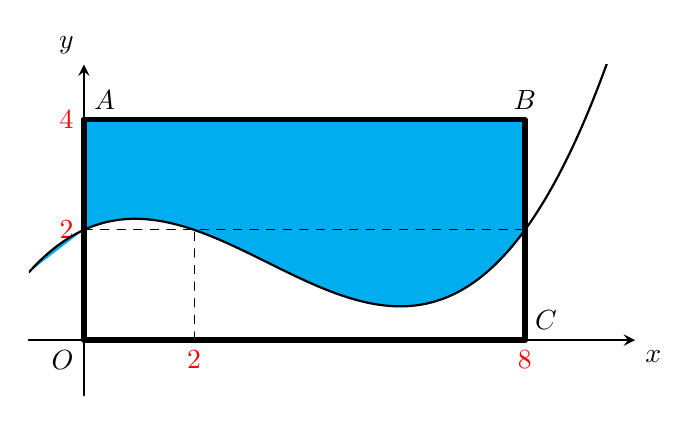
\begin{tikzpicture}[line join=round, line cap=round,>=stealth,thick,scale=0.7]
			\tikzset{label style/.style={font=\footnotesize}}
			\fill[cyan] (0,2)--plot[samples=200,domain=-1:8,smooth,variable=\x] (\x,{1/35*(\x)^3-10/35*(\x)^2+16/35*(\x)+2})--(8,4)--(0,4)--cycle;
			\draw[->] (-1,0)--(10,0) node[below right] {$x$};
			\draw[->] (0,-1)--(0,5) node[above left] {$y$};
			\draw (0,0) node [below left] {$O$};
			\foreach \x in {2,8}
			\fill[red] (\x,0) circle (1.5pt) node [below] {$\x$};
			\foreach \y in {2,4}
			\fill[red] (0,\y) circle (1.5pt) node [left] {$\y$};
			\draw[dashed,thin](2,0)--(2,2);
			\draw[dashed,thin](0,2)--(8,2);
			\draw[line width=2pt](0,0) rectangle (8,4);
			\begin{scope}
				\clip (-1,-1) rectangle (10,5);
				\draw[samples=200,domain=-1:10,smooth,variable=\x] plot (\x,{1/35*(\x)^3-10/35*(\x)^2+16/35*(\x)+2});
			\end{scope}
			\node[above right] at (0,4){$A$};
			\node[above] at (8,4){$B$};
			\node[above right] at (8,0){$C$};
		\end{tikzpicture}
	}
	\loigiai{
		Diện tích phần sơn màu trắng
		\[\left|\displaystyle\int\limits_0^8\left(\dfrac{1}{35} x(x-2)(x-8)+2\right)\mathrm{\,d}x\right|=\dfrac{1\,168}{105}. \]
		Vì $\dfrac{1\,168}{105}:4\approx 2{,}78$ nên cần mua $3$ hộp sơn màu trắng. Do đó $n=3$.\\
		Diện tích cần sơn: $S=4\cdot 8=32$ (m$^2$).\\
		Diện tích phần sơn màu xanh da trời
		\[m=S-n=32-\dfrac{1\,168}{105}=\dfrac{2\,192}{105}\ \left(\mathrm{m}^2\right). \]
		Vì $\dfrac{2\,192}{105}:4\approx 5{,}22$ nên cần mua $6$ hộp sơn màu xanh da trời. Do đó $m=6$.\\
		Vậy $m-n=6-3=3$.
	}
\end{ex}

\begin{ex}%[2D4V3-1]
	[THPT-Chuyen-LeHongPhong-HCM-NH24-25]
	Cho $(\mathscr{H})$ là hình phẳng giới hạn bởi đồ thị hàm số $y=x^2$ với $x \geq 0$, trục tung và đường thẳng $y=9$. Đường thẳng $y=a x$ chia ($\mathscr{H}$) thành hai phần có diện tích bằng nhau. Tính $a$ (làm tròn đến hàng phần chục).
	\loigiai{
		\immini{
			Giao điểm của đồ thị hàm số $y=x^2$ với $y=9$ là
			\[x^2=9\Rightarrow x=3\ (\text{do}\ x\geq 0). \]
			Diện tích hình $(\mathscr{H})$
			\[S_{\mathscr{H}}=\displaystyle\int\limits_0^3(9-x^2)
			\,\mathrm{d}x=\left(9x-\dfrac{x^3}{3}\right)\bigg|_0^3=9\cdot 3 -\dfrac{3^3}{3}=27-9=18. \]
			Vì đường thẳng $y=a x$ chia ($\mathscr{H}$) thành hai phần có diện tích bằng nhau nên diện tích mỗi phần là
			\[18:2=9. \]
			Giả sử đường thẳng $y=ax$ đi qua điểm $A(3;9)$. Khi đó diện tích phần thứ nhất là diện tích của tam giác vuông có 2 cạnh góc vuông là $9$ và $3$ và $S=\dfrac{1}{2}\cdot 9\cdot 3=13{,}5\neq 9$.\\
			Suy ra đường thẳng $y=ax$ cắt đường thẳng $y=9$.\\
			Giao điểm của đường thẳng $y=ax$ và đường thẳng $y=9$ là $B\left(\dfrac{9}{a};9\right)$.\\
			Theo đề bài, ta có phương trình
			\[\dfrac{1}{2}\cdot 9\cdot \dfrac{9}{a}=9\Leftrightarrow a=4{,}5. \]
		}{
			\begin{tikzpicture}[line join=round, line cap=round,>=stealth,thick,scale=0.8]
				\tikzset{label style/.style={font=\footnotesize}}
				\draw[->] (-1,0)--(4,0) node[below left] {$x$};
				\draw[->] (0,-1)--(0,10) node[below left] {$y$};
				\draw (0,0) node [below left] {$O$};
				\fill[pattern = north east lines,pattern color=blue]  plot[samples=200,domain=0:3,smooth,variable=\x] (\x,{1*(\x)^2+0*(\x)+0})--(0,9)node[left]{$9$};
				%	\foreach \x in {-2,-1,1,2}
				%	\draw[thin] (\x,1pt)--(\x,-1pt) node [below] {$\x$};
				%	\foreach \y in {1,2,3,4}
				%	\draw[thin] (1pt,\y)--(-1pt,\y) node [above left] {$\y$};
				\draw[dashed,thin](3,0)node[below]{$3$}--(3,9)node[above right]{$A(3;9)$}
				(2,0)node[below]{$a$}--(2,9);
				%	\draw[dashed,thin](-1,0)--(-1,1)--(0,1);
				%	\draw[dashed,thin](1,0)--(1,1)--(0,1);
				%	\draw[dashed,thin](2,0)--(2,4)--(0,4);
				\begin{scope}
					\clip (-1,-1) rectangle (4,10);
					\draw[samples=200,domain=0:3,smooth,variable=\x] plot (\x,{1*(\x)^2+0*(\x)+0})--(0,9);
				\end{scope}
				\draw (0,0)--(2,9);
			\end{tikzpicture}
		}
	}
\end{ex}

